Right clicking on a subset offers the possibility to export this subset. At the moment CSV and SDF export is supported. Starting the export will open the dialog shown in \figref{fig:export}.

\begin{figure}[!htb]
\centering
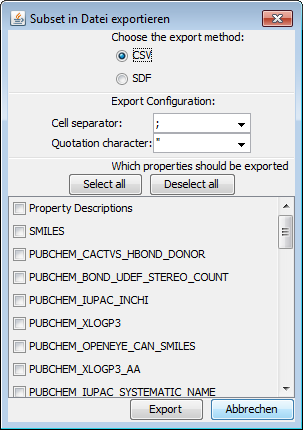
\includegraphics[width=0.4\textwidth]{images/sh_export_dialog}
\caption{Export Dialog}
\label{fig:export}
\end{figure} 

If CSV is chosen, the cell separator and the quotation character can be defined. After choosing the export format, the collection of properties which should be exported can be defined.
Clicking the export button will open a file chooser dialog to define the location and the name of the export.

After completing the export, the program will show a success message.
